\chapter{Analyse de séries de données de débits}

\section{Explication}
\begin{itemize}
    \item \underline{\textbf{Temps de retour moyens :}} 2 à 5 ans
    \item \underline{\textbf{Temps de retour rares :}} 10, 30, 100, 300 ans, \dots ! Cela dépend surtout des objectifs de protection.
\end{itemize}

\section{Séparation des crues}
\begin{figure}[H]
    \centering
    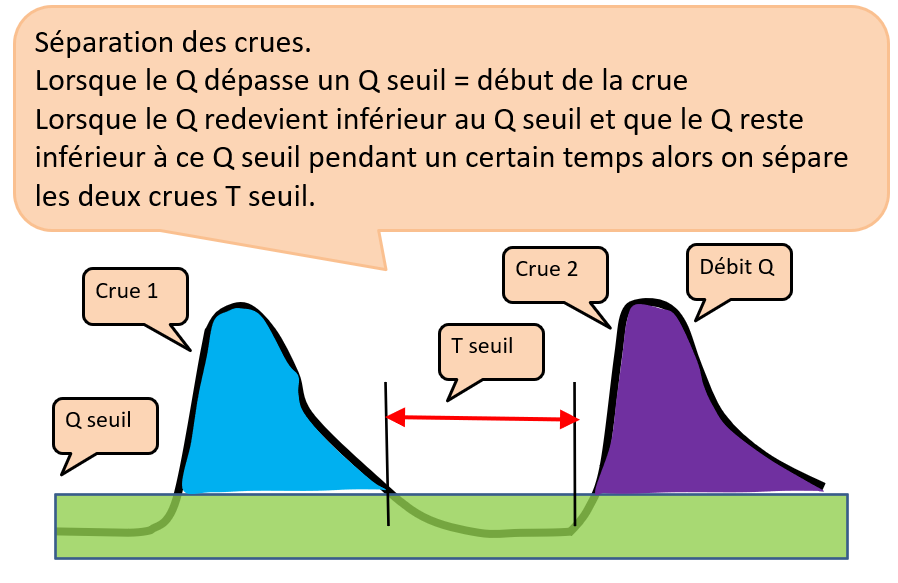
\includegraphics[width=17cm]{separationCrue.png}
    \label{fig:separationCrues}
\end{figure}

\newpage

\section{Questions intuitives sur les temps de retour}
Si on prend l'exemple suivant :
\begin{figure}[h!]
    \centering
    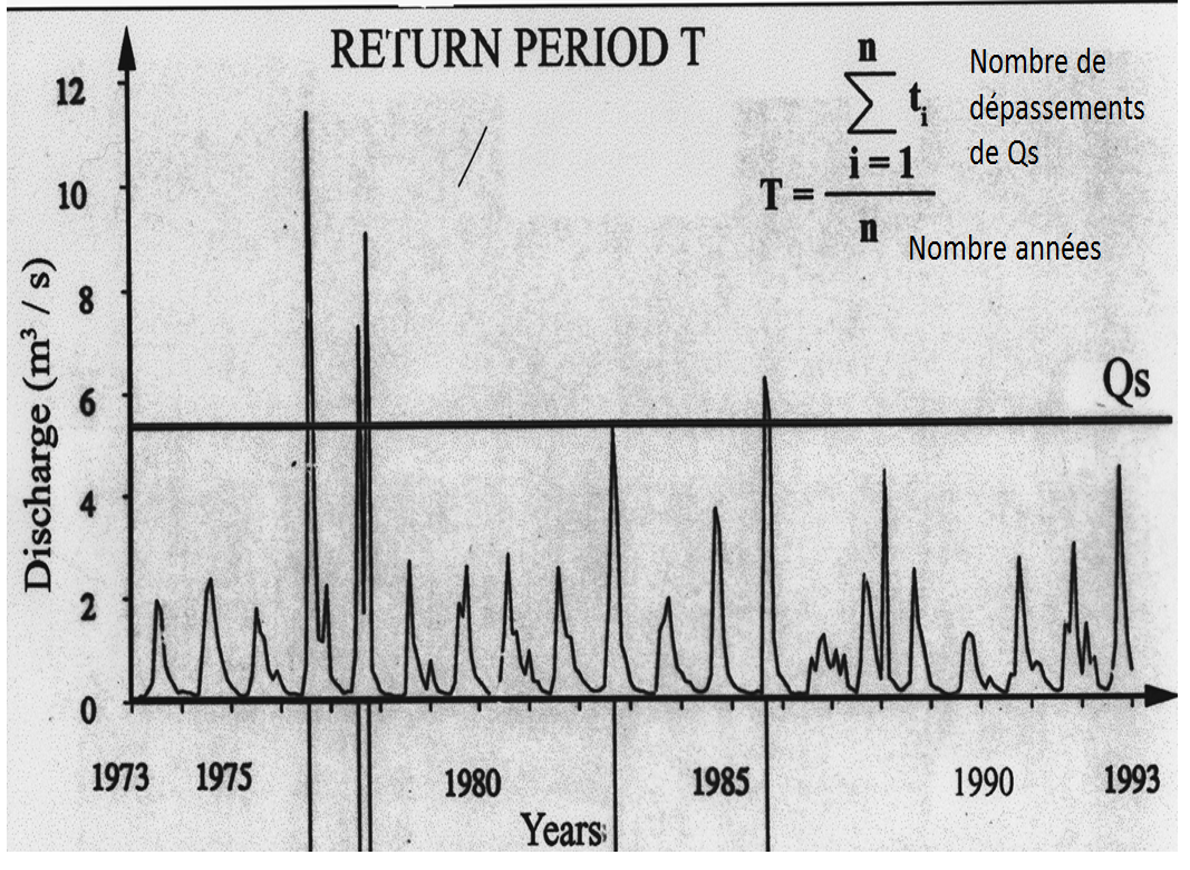
\includegraphics[width=10cm]{returnPeriodT.png}
    \caption{Graphique des débits maximums par jour}
    \label{fig:graphiqueExemple}
\end{figure}

\begin{itemize}
    \item Si on prend une période de 20 ans ; le seuil $Q_s$ est dépassé 4 fois. Donc $T_{Q_{s}} = 20/4 = 5$ ans
    \item Temps du plus gros débit : $T_{Q_{s}} = 20/1 = 20$
    \item Temps du 2\ieme ~ gros débit : $T_{Q_{s}} = 20/2 = 10$
    \item Probabilité moyenne de dépasser le plus gros débit : $P = 1/20$
    \item Probabilité moyenne de plus dépasser le plus gros débit : $F=1-(1/20)$
\end{itemize}

\paragraph{Formule de Hazen :} Questions possibles :
\begin{itemize}
    \item Avez-vous une chance de 20 ans d'observer une crue avec un T>20 ans ? \\
    \underline{Réponse :} oui 
    \item Avec la formule de Hazen, quel est le temps de retour $T$ du plus gros débit observé pendant ces 20 ans ? \\
    \underline{Réponse :} $T = \cfrac{20}{1-0.5} = 40$ ans
\end{itemize}

\section{Séries annuelles, avec débits maximaux}

\begin{itemize}
    \item On mesure un débit toutes les 10 min (exemple), tous les jours, \dots
    \item On garde les \underline{débits maximum} par an sur une \underline{période d'au moins 15 à 20 ans}.
    \item Pour extrapoler des débits de temps de retour > à la période d'observation, on applique \textbf{\underline{la loi de Gumbel} (cf. Annexe \ref{app:seriesAnnuelles}).}
\end{itemize}

\subsection{Stationnarité}
\begin{itemize}
    \item Permet de vérifier si les données ne varie pas dans le temps.
    \item Ce contrôle de l'évolution des crues de pointes donne un aperçu d'une dérive s'il y a.
    \item Si elles ne le sont pas, on ne pourra pas extrapoler de valeurs pour des temps de retour de 50 ans par ex.
\end{itemize}

\subsection{Homogénéité}
\begin{itemize}
    \item Il est bon de contrôle l'homogénéité des données quand c'est possible (débit maximal par mois)
    \item On trace une courbe par an, en fonction des mois.
    \item Ces courbes doivent être semblable puisqu'elle résulte d'un même processus météorologique (ex : pluies ou fonte des neiges).
    \item Effets anthropiques pertubateurs comme les barrages, ou des épisodes isolés comme des ruptures de barrages 
\end{itemize}

\section{Séries gonflées}
Une série gonflée est une série de données statistiques où nous avons \underline{2 ou plus débits maximaux par année}. \\
Il faut faire attention car parfois on prend des crues très petites pour des années très sèches alors que d'autres années, ces mêmes crues sont atteintes ou dépassées plusieurs fois ! \\
\textbf{Privilégiez les séries tronquées}

\section{Séries tronquées}
Une série tronquée est une série de données statistiques où les \underline{débits sont supérieurs à $Q_\text{seuil}$.} \\
\Warning Si le seuil est trop bas, on prend des débits très fréquents et des débits extrêmes ; qui ne sont peut-être pas homogènes. \\
On prend les séries tronquées pour obtenir les débits fréquents de temps de retour faible; voire inférieur au temps de retour de l'an. \\
Privilégiez les séries tronquées aux séries gonflées. \\
\Warning La notion à prendre en compte lors de l'ajustement par la loi de Gumbel est le nombre de valeurs de temps de retour.
On va calculer des temps de retour très bas (< 1 an), ce qui va peser un certain poids sur la courbe de tendance\dots